% Appendix D, Figure D.1 --- "The tetrahedral POVM, end to end".  The layout only.
%
% Layout: card_oct_body.tex's header is binding.  Deviations from it, and only
% they, are listed here.
%
%   * the sphere is Figure 1.1's own recipe_tet_sphere.pdf, reused byte for
%     byte rather than redrawn, so that Figure 1.1 and this card agree by
%     construction instead of by luck.  Assertion 21 measures whichever file
%     is named, so the reuse is checked and not exempted.
%   * the circuit is the widest of the five relative to its content
%     (336.465bp) and the side stack the tallest (four atoms: $U_A$, $\alpha$,
%     $\beta$, and $S$ with $H$), so band 2 runs 344pt + 103pt.
%   * BAND 4 HAS NO RAY LIST.  These four vertices form no antipodal pair, so
%     there is no coin: head 4 reads "No coin over axes" and the band is one
%     label.  Its first sentence is the only place on the five cards where
%     the two randomized protocols meet, and they must meet as a contrast --
%     without it a reader concludes this solid admits no randomization at
%     all, which its own dashed $U_g$ contradicts one band above.  Its
%     second sentence is the one claim on the five pages that bsc-thesis.tex
%     makes nowhere else: draw 2T against an aligned vertex anyway and the
%     readout's two poles assemble the CUBE, eight effects of weight 2/8.
%     Not a failure -- a different POVM, and the only Platonic case where
%     the vertex orbit is not already antipodally closed.  It is also this
%     card's one outward pointer, to Figure D.3.  Head 4 carries no Appendix
%     A pointer: there are no coin words to route.
%   * the reserve is 171.63pt, the largest of the five by a wide margin, and it sits
%     below the caption as trailing white.  The tetrahedron IS the small card
%     -- four vertices, two wires, no dead outcome, no coin -- and Figure 1.1
%     already carries it in full.
% All macros below are \def and therefore local to the figure environment.
\parindent=0pt \parskip=0pt
% Auto-generated by code/_build_povm_cards.py -- DO NOT EDIT.
% The data blocks of the tetrahedral card of Appendix D
% (paper/figures/card_tet_body.tex \input's this and calls them).  Every
% number is derived from code/data/*.npz, Decker's circuits as
% randomized_decker rebuilds them, Figure 1.1's own \RecipeSeriesStrip, and
% Tables E.1, 5.2, D.1, D.3 and D.4, and is checked back against them before
% this file is written; see the builder's docstring for the checks (and
% _povm_cards_controls.py, which shows each of them failing on one corrupted
% literal: 100 negative controls, all aborting, 0 stale).
% Requires: booktabs, mathtools, hyperref, and the thesis macros \Id, \pmat,
% \bra, \ket, \braket, \Tr, \C, \sigmavec, \TwoT, \TwoO, \TwoI, \phig,
% \invphig, \sigmaz.  The body defines \NIS, \CTR, \PBOX, \COL, \FULLHEAD,
% \BANDRULE and \TAB, which \CardSide and the tables use.
% Regenerate with `cd code && uv run _build_povm_cards.py`.

\newcommand{\CTitle}{The tetrahedral POVM, end to end}
\newcommand{\CPtrStrip}{Introduction reference: Figure~\ref{fig:tetrahedron-recipe}}
\newcommand{\CHeadA}{Vertices and effects, $E_k = \tfrac1V(\Id + \hat n_k \cdot \sigmavec)$.}
\newcommand{\CPtrA}{Table~\ref{tab:povm-atlas} $\cdot$ Equation~\eqref{eq:povmform}}
\newcommand{\CHeadB}{Circuit; the dashed $U_g$ is an optional prepended rotation.}
\newcommand{\CPtrB}{Section~\ref{subsec:rotated-povms} $\cdot$ Table~\ref{tab:decker-pose}}
\newcommand{\CHeadC}{Register $\to$ vertex, top wire first}
\newcommand{\CPtrC}{Table~\ref{tab:decker-labels} $\cdot$ Section~\ref{sec:decker:using}}
\newcommand{\CHeadD}{No coin over axes}
\newcommand{\CPtrD}{Table~\ref{tab:decker-vs-coin} $\cdot$ Section~\ref{subsec:randomized-implementations}}

\newcommand{\CStrip}{{\footnotesize\setlength{\tabcolsep}{4pt}\renewcommand{\arraystretch}{0.88}%
\begin{tabular}{@{}c c c c l l l@{}}
\toprule
$V$ & group & anc. & dead & reorientation exact? & relabelling & \hyperref[tab:decker-vs-coin]{coin over axes}\\
\midrule
4 & $\TwoT$ & 1 & 0 & $T^\dagger$, over Clifford${}+T$ & identity & none: no antipodes\\
\midrule
\multicolumn{7}{@{}l@{}}{only the octahedral coin is exact --- this dilation is not (Theorem~\ref{thm:main}, Appendix~\ref{sec:decker:exactness})}\\
\bottomrule
\end{tabular}}}

\newcommand{\CardVertexTable}{%
\begin{tabular}{@{}r l c r@{}}
\toprule
$k$ & $\hat n_k$\ $(\times\tfrac{1}{\sqrt3})$ & $E_k\ (\times\tfrac{\sqrt3}{12})$ & $\bra{0}E_k\ket{0}$ \\
\midrule
$1$ & $(+1,\,+1,\,+1)$ & $\pmat{\sqrt3+1 & 1-i \\ 1+i & \sqrt3-1}$ & $0.3943$ \\ \addlinespace[3pt]
$2$ & $(-1,\,-1,\,+1)$ & $\pmat{\sqrt3+1 & -1+i \\ -1-i & \sqrt3-1}$ & $0.3943$ \\ \addlinespace[3pt]
$3$ & $(-1,\,+1,\,-1)$ & $\pmat{\sqrt3-1 & -1-i \\ -1+i & \sqrt3+1}$ & $0.1057$ \\ \addlinespace[3pt]
$4$ & $(+1,\,-1,\,-1)$ & $\pmat{\sqrt3-1 & 1+i \\ 1-i & \sqrt3+1}$ & $0.1057$ \\ \addlinespace[3pt]
\bottomrule
\end{tabular}
}

\newcommand{\CIdent}{$\sum_k E_k = \Id$, $\Tr E_k = \tfrac12$, rank one, a $2$-design; $|\braket{\psi_j}{\psi_k}|^2 = \tfrac13$ for $j \neq k$: the SIC condition.}
\newcommand{\CIdentB}{}

\newcommand{\CParams}{$U_R$ inverts Table~\ref{tab:decker-pose}'s $R$; a drawn $U_g$ twirls and relabels outcomes by $g^{-1}$.\par\vskip1pt $Q^\dagger$: the CNOT $\ket{00}\mapsto\ket{00}$, $\ket{11}\mapsto\ket{01}$; the ancilla-controlled $S$ realizes $\mathrm{diag}(1,1,1,i)$\par\vskip1pt $\tilde{M}^\dagger = (I_2 \otimes \mathsf{F}_2)\,\mathrm{diag}(1,1,1,i)\,(U_A \otimes I_2)\,Q^\dagger$, the Naimark extension unitary the solid box implements}

\newcommand{\CardSide}{\CTR{\hsize}{$U_A = \sqrt2\,\pmat{\alpha & \beta \\ \beta & -\alpha}$}\NIS{4pt}\CTR{\hsize}{$\alpha = \sqrt{(3+\sqrt3)/12}$}\NIS{4pt}\CTR{\hsize}{$\beta = \sqrt{(3-\sqrt3)/12}$}\NIS{4pt}\CTR{\hsize}{$S = \mathrm{diag}(1,i)$, $H = \mathsf{F}_2$}}

\newcommand{\CardKey}{%
\begin{tabular}{@{}c c c@{}}
\toprule
& \multicolumn{2}{c}{\footnotesize lower} \\
{\footnotesize upper} & $\mathtt{0}$ & $\mathtt{1}$ \\
\midrule
$\mathtt{0}$ & 1 & 2 \\
$\mathtt{1}$ & 3 & 4 \\
\bottomrule
\end{tabular}
}

\newcommand{\CKappa}{Run $U_R$ and read the key, or skip $U_R$ and read Decker's own numbered list~\cite{decker2004quantumcircuitssinglequbit}: either way $\kappa = 1$, free. His circuit with our list, index for index, is the mismatch: $\kappa = +0.804738$; under the drawn twirl it costs a $1/\kappa^2 = 1.54\times$ premium in shots, never a bias.}

\newcommand{\CRays}{}

\newcommand{\CCoin}{The dilation is forced; a drawn $U_g$ still twirls it. Align a vertex and draw from $\TwoT$ anyway: each readout reports an axis, not a vertex, and the eight effects assembled are the cube's (Figure~\ref{fig:dec_cube_circuit}).}

\long\def\NIS#1{\vskip #1\nointerlineskip}
\long\def\CTR#1#2{\hbox to #1{\hss #2\hss}}
\long\def\PBOX#1#2{\vtop{\hsize=#1\parindent0pt\sloppy\emergencystretch=1.5em\small #2}}
\long\def\COL#1#2{\vtop{\hsize=#1\parindent0pt\hbox{}\nointerlineskip #2}}
\long\def\FULLHEAD#1#2#3{\hbox to \hsize{\small\textbf{#1}\,#2\hfil{\footnotesize #3}}}
\def\BANDRULE{\vskip2pt\hrule height0.5pt\vskip1.5pt\nointerlineskip}
\long\def\TAB#1{{\small\renewcommand{\arraystretch}{0.88}\setlength{\tabcolsep}{3pt}#1}}
%
\vbox{\hsize\textwidth\parindent0pt
%
% --- title and the header strip: Figure 1.1's own row -----------------------
\hbox to \hsize{\large\bfseries \CTitle\hfil{\normalfont\footnotesize \CPtrStrip}}%
\NIS{5pt}%
\hbox{\CStrip}%
\BANDRULE
%
% --- band 1: the object -----------------------------------------------------
\FULLHEAD{1}{\CHeadA}{\CPtrA}%
\NIS{5pt}%
\hbox to \hsize{%
  \COL{170pt}{\CTR{170pt}{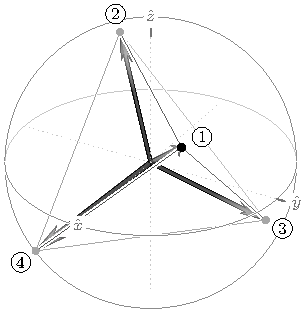
\includegraphics{figures/recipe_tet_sphere.pdf}}}%
  \hfil
  \COL{277pt}{\hbox to 277pt{\hfil\TAB{\CardVertexTable}}}%
}%
\NIS{4pt}%
\PBOX{\hsize}{\CIdent}%
\BANDRULE
%
% --- band 2: the machine ----------------------------------------------------
\FULLHEAD{2}{\CHeadB}{\CPtrB}%
\NIS{5pt}%
\hbox to \hsize{%
  \COL{344pt}{\hbox to 344pt{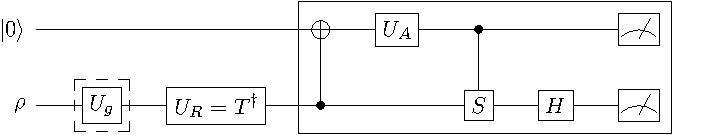
\includegraphics{figures/card_dec_tet.pdf}\hss}}%
  \hfil
  \COL{103pt}{\small\CardSide}%
}%
\NIS{5pt}%
\PBOX{\hsize}{\CParams}%
\BANDRULE
%
% --- band 3: the readout ----------------------------------------------------
\FULLHEAD{3}{\CHeadC}{\CPtrC}%
\NIS{5pt}%
\hbox to \hsize{%
  \COL{120pt}{\TAB{\CardKey}}%
  \hfil
  \COL{324pt}{\PBOX{324pt}{\CKappa}}%
}%
\BANDRULE
%
% --- band 4: the alternative ------------------------------------------------
\FULLHEAD{4}{\CHeadD}{\CPtrD}%
\NIS{5pt}%
\PBOX{\hsize}{\CCoin}%
}%
